\documentclass[10pt,draftcls,twocolumn]{IEEEconf}
\usepackage[utf8]{inputenc}
\usepackage{graphicx}


% Title Page
\title{Loss recovery with tail loss probe in Multipath TCP}
\author{KAU}

\begin{document}
\maketitle

\begin{abstract}
Packet losses are a well known cause of performance hindrance in the Internet. Transport protocols recover from the packet losses in order to provide reliable end to end communication. The efficiency
of loss recovery greatly influences the completion time of the flows. In this paper we focus on the state of the art los recovery mechanisms for TCP and Multipath TCP. We use controlled tail loss scenarios
to calculate the burst completion time. We propose an enhancement to the tail loss recovery in Multipath TCP. Our experiment results show performance improvement in controlled scenarios. 
\end{abstract}

\section{Introduction}


Multipath TCP is an experimental standard proposed as an extension to TCP~\cite{rfc6824}. It allows devices with multiple interfaces to transmit simultaneously on both interfaces.  
In Multipath TCP(MPTCP), a connection can have multiple TCP sub flows using different interfaces on different routes. Each TCP subflow imparts the functional behavior of a standard TCP flow. 
MPTCP uses a connection level congestion window as well as sub flow level congestion windows for each sub flow. Packet losses in each sub flow are detected and recovered in a similar fashion as that of TCP. However, It is not restricted in the standard on how the loss recovery happens in the implementation and which sub-flow retransmits the lost packets. If the recovery is handled at the meta level, the lost packet may be rescheduled and retransmitted at the available sub flow with lowest RTT. If the recovery is handled at the flow level, the packet may be retransmitted in the same sub-flow. An important part of this recovery process is to follow the TCP semantics. 

TCP has two mechanisms for detecting and recovering from packet losses namely Fast Recovery (FR) and Retransmission Timeouts(RTOs). Fast recovery is triggered on receipt of predecided number of duplicate acknowledgements, considering it as a loss indication. RTOs wait for the packet loss to trigger a timeout for retransmitting that packet. For long flows where there are sufficiently large number of packets to be transferred, FR is quicker than RTOs in detecting and recovering packet losses. On the other hand shorter flows which are a majority in the web traffic have to depend on RTOs for packet loss detection and recovery thus incurring more latency. A single packet loss in a short flow may take many RTTs to detect and recover. This scenario is also applicable to the packets at the end of the flow (or tail) in a long flow.

TCP Loss Probe (TLP)~\cite{Flach:2013} a mechanism that allows flows to detect and recover from tail losses much faster than an RTO, thereby speeding up short transfers. With TLP a packet loss in the middle 
of a packet train as well as at the tail end will now trigger the same fast recovery mechanisms. It assumes other algorithms such as early retransmit~\cite{rfc5827} and FACK threshold based recovery are 
present.


Retransmission schemes of TCP are of significant importance in achieving lower flow completion times. TLP is the recent scheme proposed and implemented in Linux kernel. Further 
evaluationsin~\cite{Rajiullah:2015}, showed that TLP provides significant reductions in latency for short flows with one to n-degree tail losses. In this paper we provide the related research on retransmission in section~\ref{relwork} leading to the experimental setup.

\section{Background and Related Work}\label{relwork}

Multipath TCP uses two levels of sequence numbers to support efficient data transfer, namely data sequence and TCP sequence. Data sequence is for the end to end data transfer and TCP sequence number is for individual flow data sequence similar to TCP. A loss occurring in an individual TCP flow corresponds to a loss in end to end data. Multipath TCP, as an extension of TCP, uses the basics of TCP retransmission. However, the interaction with two levels makes the problem of retransmission more challenging than in TCP. The dual sequence numbering enables MPTCP to respond to loss of packets or loss of subflows by retransmitting the lost packets on an alternate path. It allows a packet to be retransmitted on a different subflow than that of the originally sent flow. The Linux implementation of MPTCP uses a set of retransmission heuristics to decide on the retransmissions. The data outstanding on timed out subflows should be rescheduled for transmission on different subflows using first timeout as the indicator. Fast retransmit on a subflow will not trigger retransmission on another subflow. It is often the case in MPTCP connection that there is path asymmetry among the subflow characteristics. Authors in~\cite{fuso}, try to exploit the path diversity by quickly retransmtting on the fast paths. 



\section{Scope}\label{scope}

This paper analyzes the performance of state of the art loss recovery mechanism of MPTCP and presents case for improvement in the tail loss scenario. 
For understanding the loss recovery and retransmission policies in MPTCP linux implementation version 0.91, we consider specific cases of tail losses.  
No tuning of TCP settings performed such as adjusting the delayed ACK behavior or time and flip on Nagle algorithm. We consider the standard settings
of Linux kernel. In the following experiments, we do not consider the congestion control interaction with the retransmission. We consider mainly failure
induced packet loss and its recovery.

\section{Experimental Setup}\label{exsetup}

Experiments use CORE emulation platform with a simple topology as depicted in Figure~\ref{fig1}.
Client is connected to two wireless interfaces 3G/4G and WLAN. Server is connected to a wired router.
Characteristics of the connection setup and assumptions about the parameters are provided in table~\ref{tab1}.
There is no attempt in this study to focus on the effect of link characteristics in retransmission performance.
 
\begin{figure}[!ht]
\begin{center}
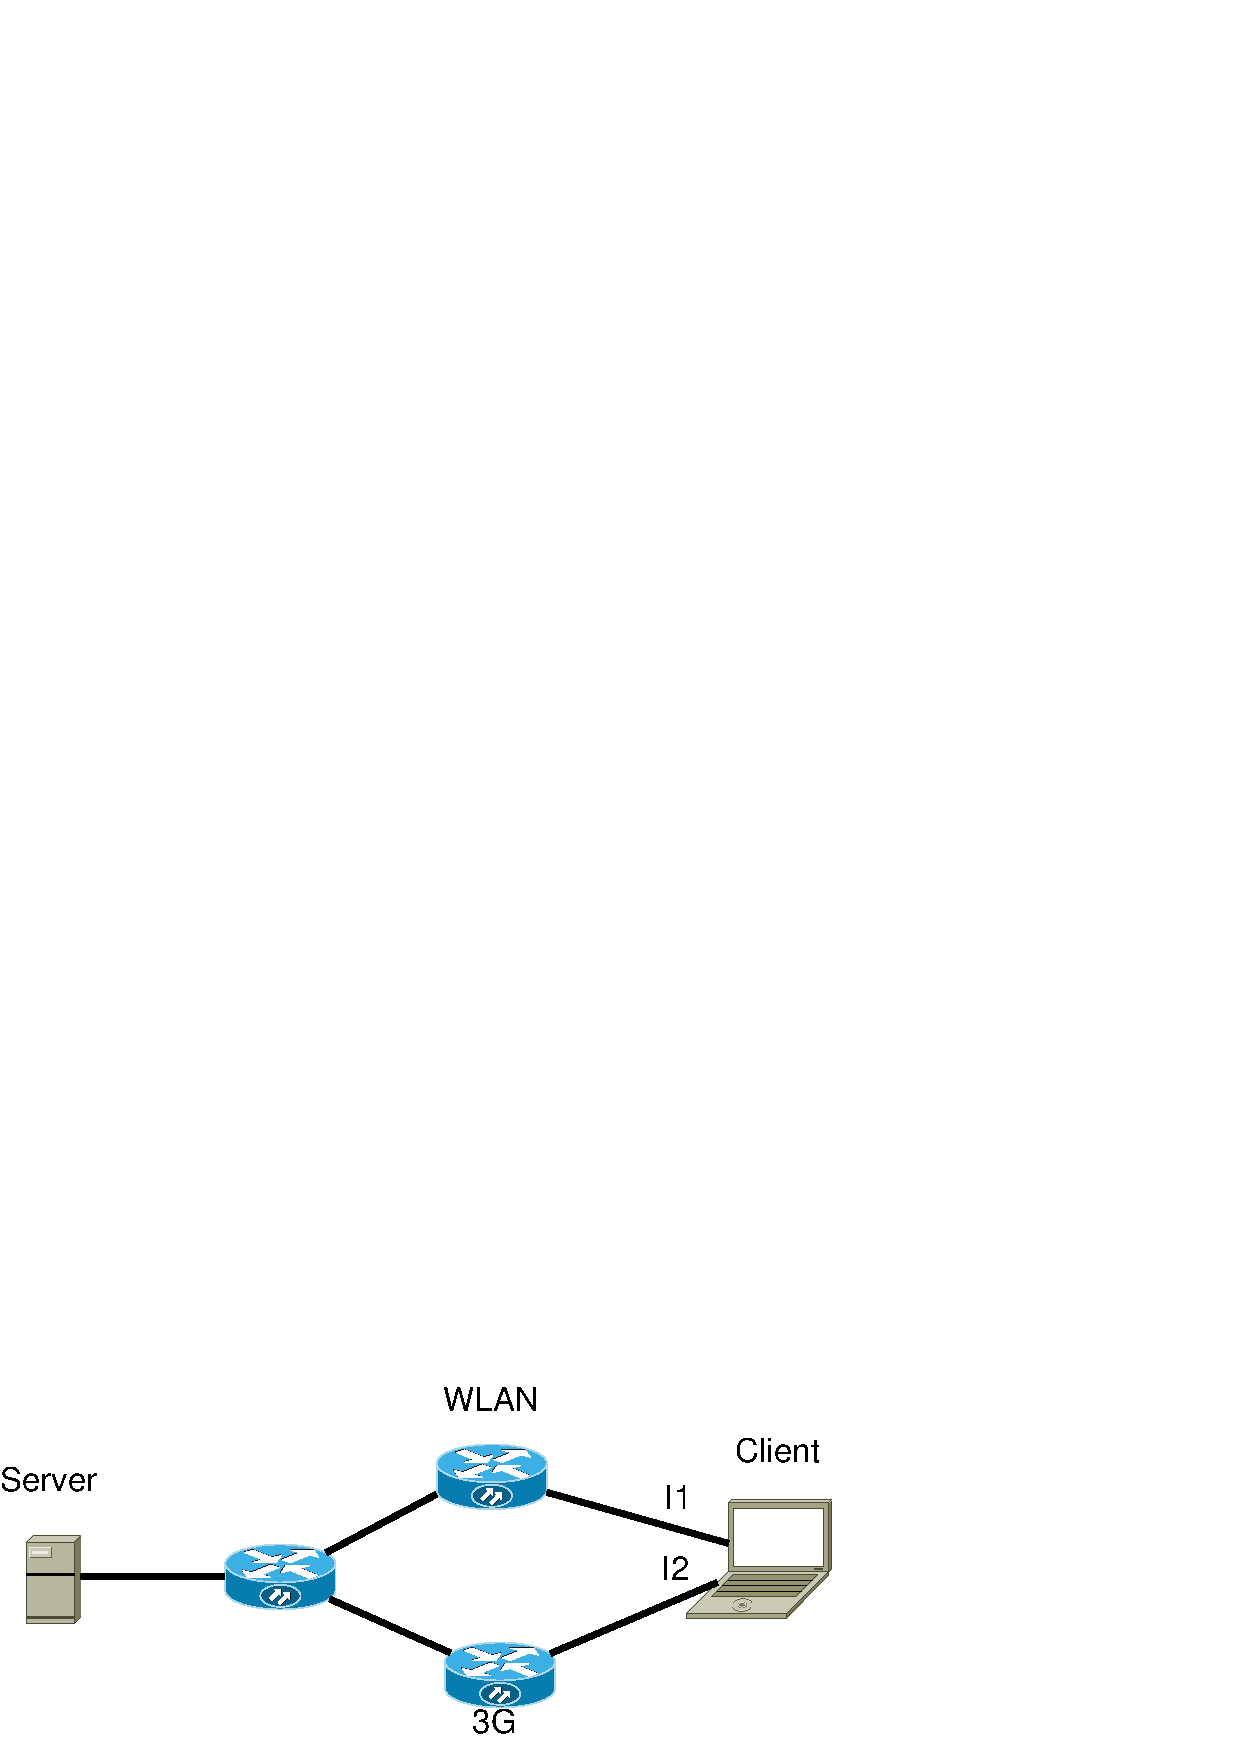
\includegraphics[angle=0, width=0.45\textwidth]{images/fortest.pdf}
\caption{Topology used for Emulation}\label{fig1}
\end{center}
\end{figure}
\begin{center}

\begin{table}
\resizebox{0.45\textwidth}{!}{\begin{minipage}{0.45\textwidth}
\small
\begin{center}
\begin{tabular}{|c|cccccccccc|}
      \hline
      
      \multicolumn{1}{c}{} & & \\[\dimexpr-\normalbaselineskip-\arrayrulewidth]
      \textbf{Burst Size} & \multicolumn{10}{c|}{80 Packets} \\
      \hline
      \textbf{Separation Time} & \multicolumn{10}{c|}{2s} \\
      \hline

      \textbf{RTT} & \multicolumn{10}{c|}{20ms-120ms(3G/4G/WLAN)}  \\
      \hline 	
      \textbf{Bandwidth} & \multicolumn{10}{c|}{54Mbps(3G/4G/WLAN)}  \\
      \hline
      \textbf{Loss Model} & \multicolumn{10}{c|}{Deterministic}\\
      \hline
      	
\end{tabular}
\caption{Connection parameters}\label{tab1}
\end{center}
\end{minipage}}
\end{table}
\end{center}


\subsection{Testing retransmission with deterministic loss patterns}
In order to understand the retransmission behavior of the Linux MPTCP implementation and to reproduce the observed retransmissions, we use a deterministic drop pattern.
Losses generated by using associating netem with corresponding interfaces and dropping the packets. This process is simplified by using the KAUNetem tool~\cite{Garcia2016}. 
MPTCP connection starts with a single TCP subflow and subsequently, one or more subflows are added following an agreement between client and server on the MPTCP protocol 
support and interface availability. So one has to wait in time and packets for the second subflow establishment to understand the MPTCP retransmissions. We send two bursts of 80 
packets each and drop tail packets on one of the interface. This is to ensure that the necessary and sufficient conditions for probe triggering are met and tail loss probe is generated on that
subflow. Three test cases are evaluated with one packet tail loss, two packet tail loss and  one packet along with probe loss. 

In Linux, TCP retransmission features are controlled by a sysctl setting tcp.early.retrans. It has 5 possible values with ranging from 0 to 4 with 3 being Linux default, enables both
ER and TLP. Standard TCP used by other operating systems might not use ER and TLP. We use RTO to refer sysctl setting of 0 and TLP to refer sysctl setting of 3 throughout the paper.
In standard TCP (RTO), disabling ER and TLP gives the performance of RTO. In Linux default TCP, enabling delayed ER gives the combined performance of RTO, delayed ER and TLP.
In standard TCP, probe loss scenario is equivalent to lossing the retransmitted packet.

In each setting, we calculate burst completion time for two bursts of 80 packets each. The setup has server and client with Linux supporting MPTCP running on them. Client has two wireless 
interfaces with one way delay on each interface ranging from 20ms to 120ms. We consider 5 scenarios with delay pairings 20ms-20ms, 20ms-30ms, 20ms-120ms, 30ms-20ms, 120ms-20ms to understand 
the effect of delay difference in the performance. These scenarios are choosen to evaluate the effect of symmetry, mild asymmetry and higher asymmetry in link delays. 

\section{Observations and Discussion}\label{disc}
This section provides the performance analysis of TCP and MPTCP for the considered cases of single packet tail loss, retransmission or probe loss and two packet 
tail loss.

\subsection{TCP}
Retransmission behavior of TCP provides a base case for MPTCP performance as each individual MPTCP subflow is a TCP flow in itself. Our analysis
starts with the results using TCP and compares it with that of the MPTCP. Figures ~\ref{t1p},~\ref{t2p},~\ref{t1pp} represent the comparison of TCP 
burst completion times. Path asymmetry is irrelevant as the TCP uses single path.

In the case of single packet tail loss, there is no difference in burst completion times of RTO and TLP settings. TLP implementation in linux accounts
for the delayed ACK and waits 200ms before sending probe. Hence retransmission timeout is the mode of loss recovery in both RTO and TLP. This can be avoided by tuning
the ACKs as discussed in~\cite{Rajiullah:2015}.
In the case of two packet tail loss, TLP performs better than RTO as it employs a combination of TLP and ER to recover from losses. 
If the probe or retransmission is lost, then TLP still performs better than STD as it waits for one RTO and one probe timeout instead of two RTOs.

\begin{figure}[!ht]
\begin{center}
\includegraphics[angle=0, width=0.46\textwidth,natwidth=578.16,natheight=433.62]{plots/T1P.pdf}
\caption{Single packet tail loss using TCP}\label{t1p}
\end{center}
\end{figure}



\begin{figure}[!ht]
\begin{center}
\includegraphics[angle=0, width=0.46\textwidth,natwidth=578.16,natheight=433.62]{plots/T2P.pdf}
\caption{Two packet tail loss using TCP}\label{t2p}
\end{center}
\end{figure}


\begin{figure}[!ht]
\begin{center}
\includegraphics[angle=0, width=0.46\textwidth, natwidth=578.16,natheight=433.62]{plots/T1PP.pdf}
\caption{Single packet tail loss together with probe loss using TCP}\label{t1pp}
\end{center}
\end{figure}

\subsection{MPTCP}


The expected retransmission behavior of MPTCP for standard TCP and Linux default settings is shown 
in~\ref{timing1P},~\ref{timing1PP} and ~\ref{timing2P}. The actual pattern might differ in cases,
where the RTT is larger than 200ms. 

\begin{figure}[!ht]
\begin{center}
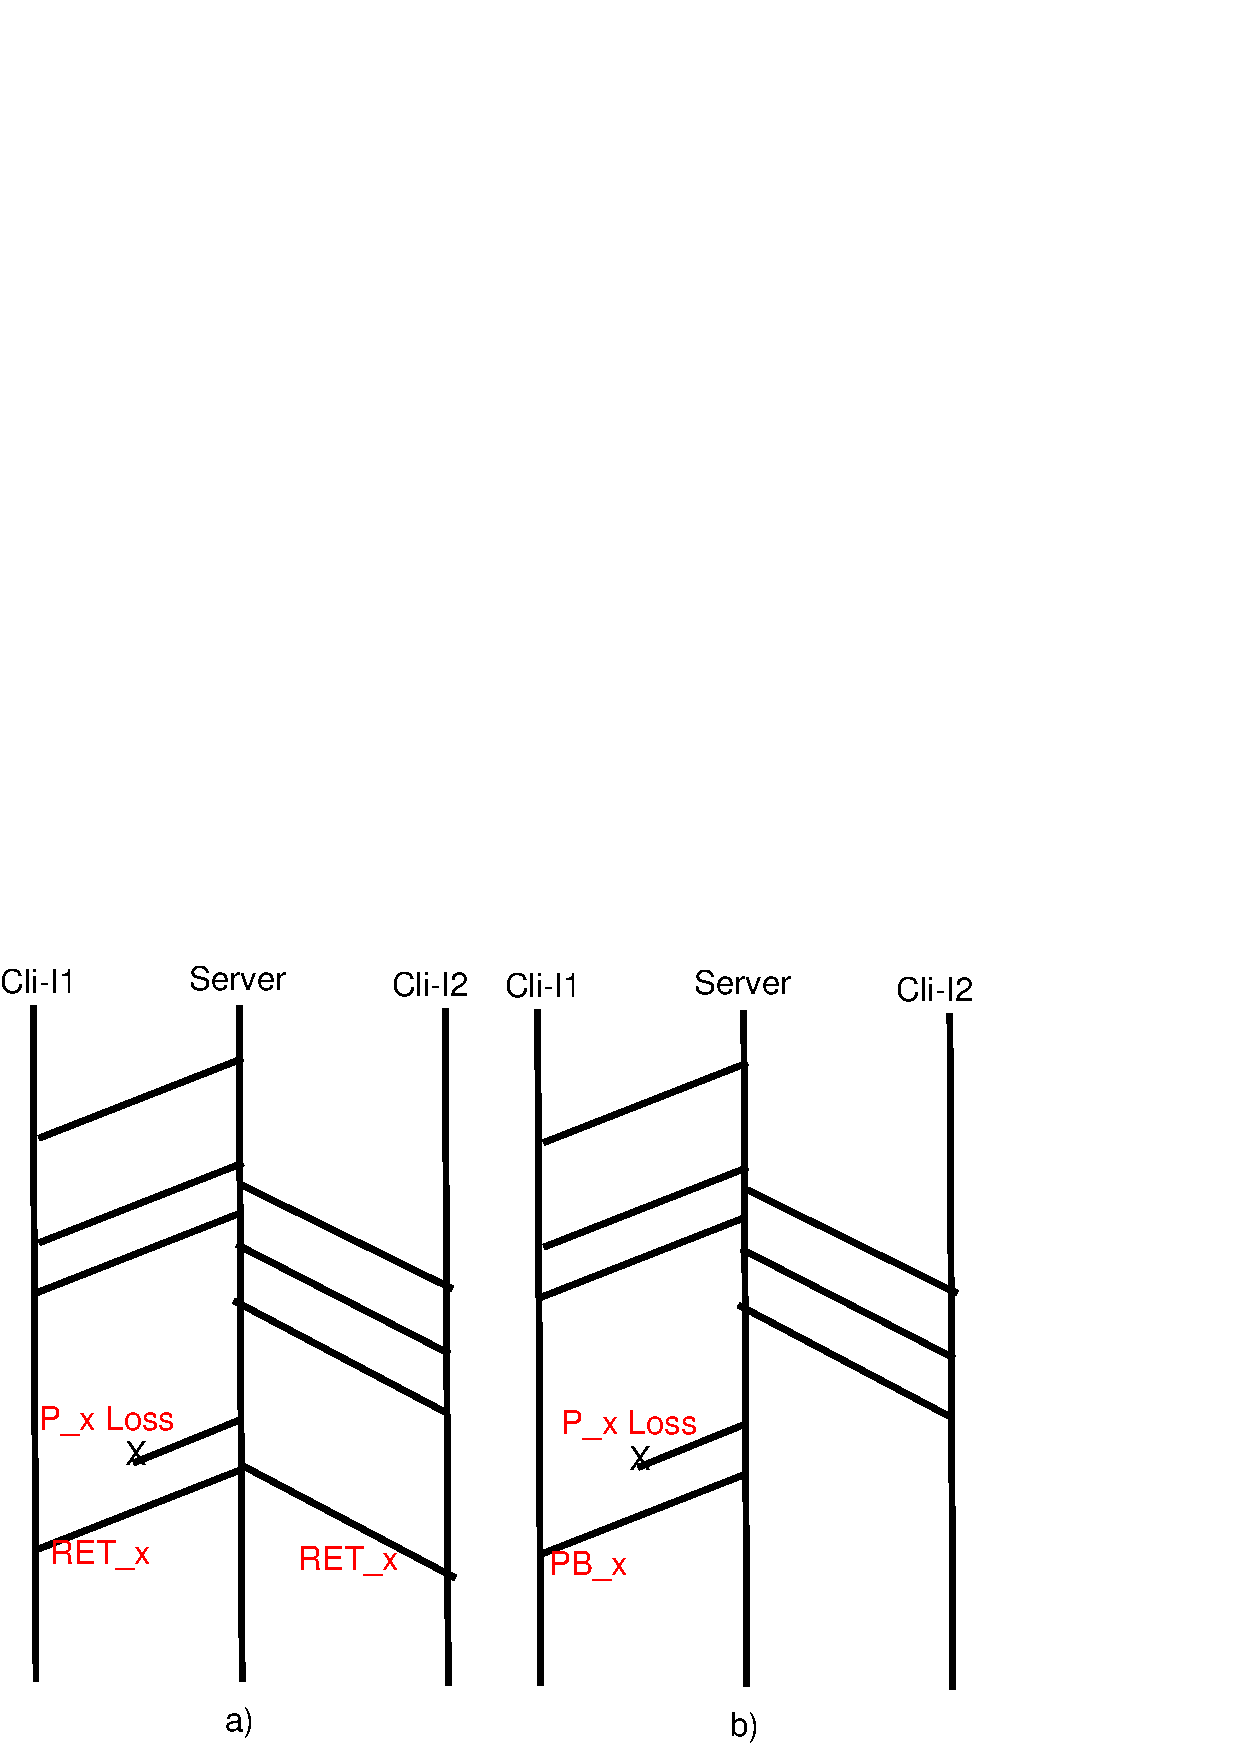
\includegraphics[angle=0, width=0.45\textwidth, natwidth=610, natheight=400]{images/timing1P.pdf}
\end{center}
\caption{Timing diagram of MPTCP behavior with one packet tail loss a) RTO b) TLP}\label{timing1P}
\end{figure}

\begin{figure}[!ht]
\begin{center}
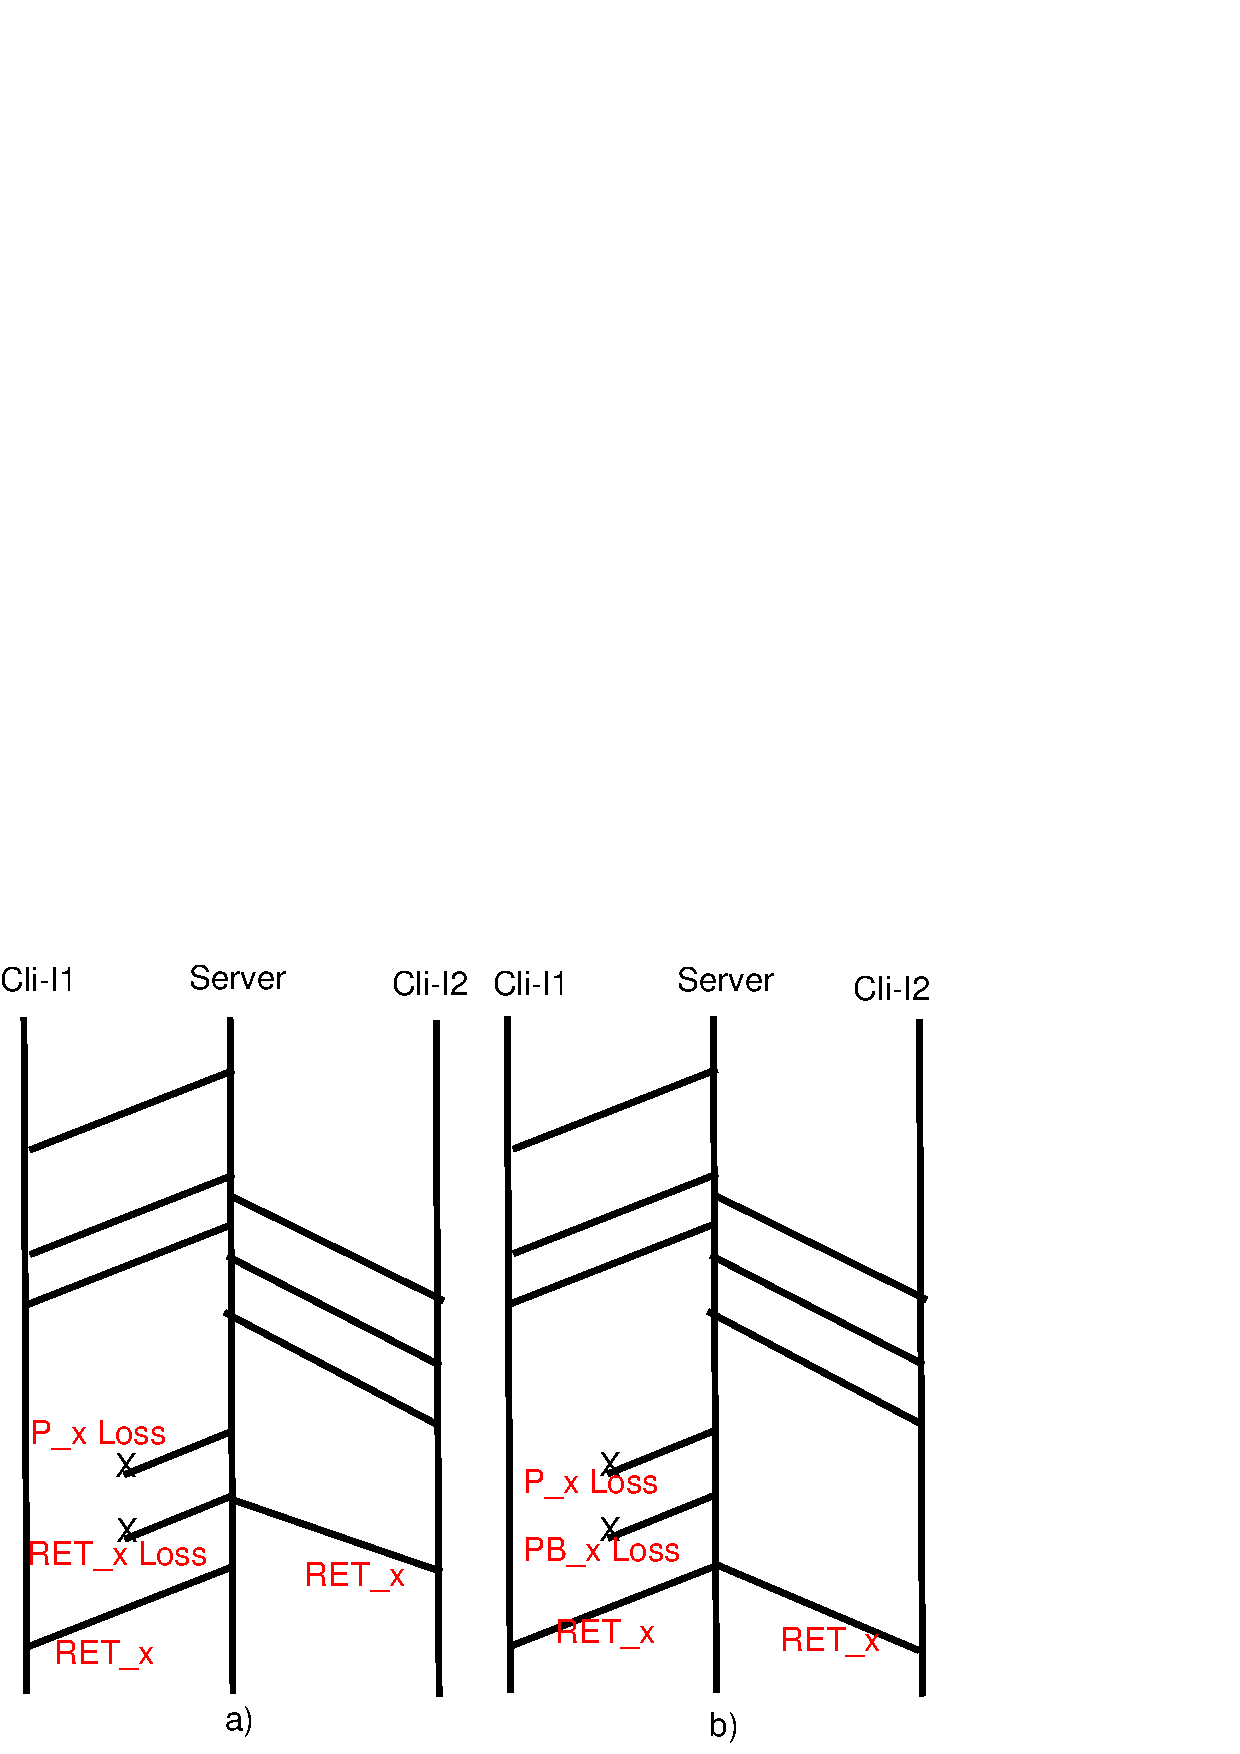
\includegraphics[angle=0, width=0.45\textwidth, natwidth=610, natheight=400]{images/timing1PP.pdf}
\end{center}
\caption{Timing diagram of MPTCP behavior with one packet and next probe loss a) RTO b) TLP}\label{timing1PP}
\end{figure}

\begin{figure}[!ht]
\begin{center}
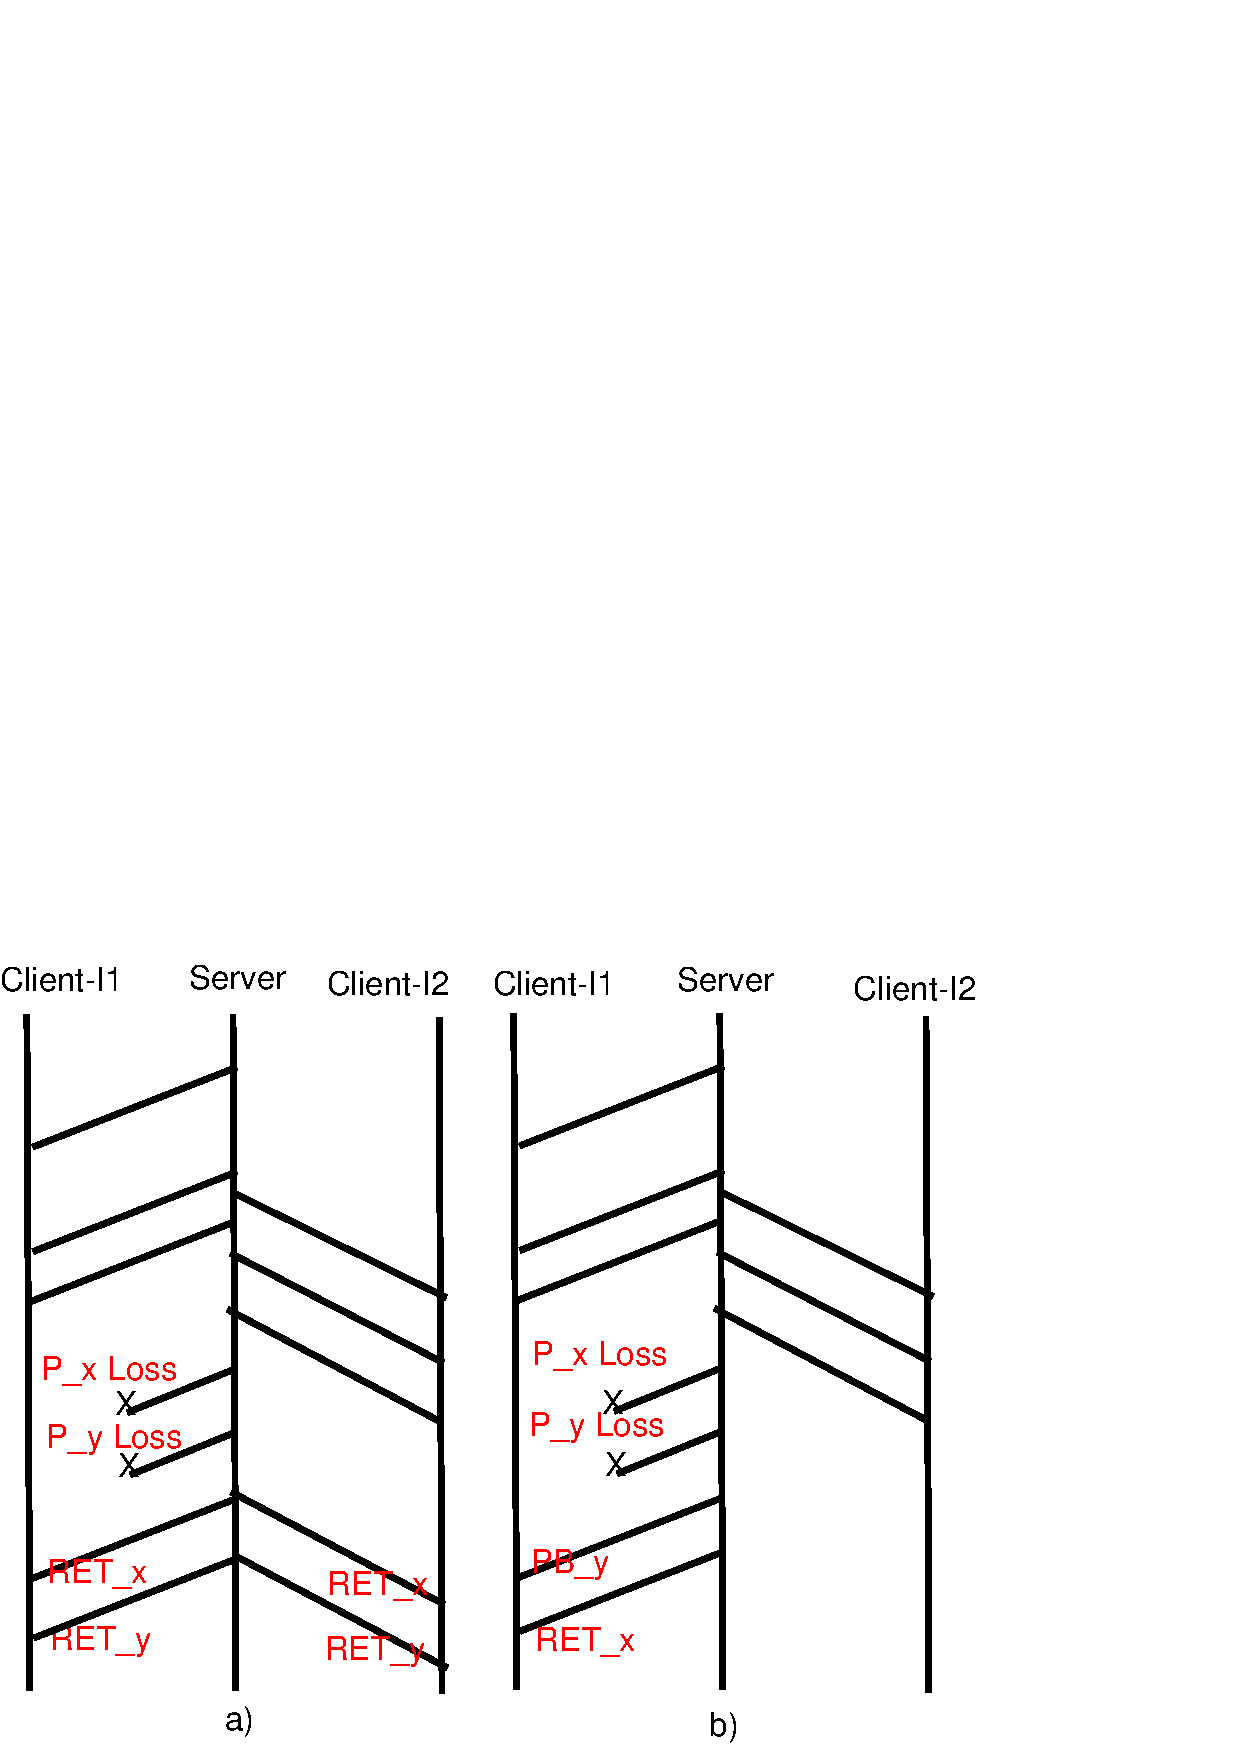
\includegraphics[angle=0, width=0.45\textwidth, natwidth=610, natheight=400]{images/timing2P.pdf}
\end{center}
\caption{Timing diagram of MPTCP behavior with two packet tail loss a) RTO b) TLP}\label{timing2P}
\end{figure}



Experiments performed on CORE emulator with the setup mentioned in section\ref{exsetup}.
MPTCP is sensitive to path asymmetry in general due to the default scheduler being shortest RTT based scheduler.

The burst completion times on single packet tail loss calculated for each delay configuration and retransmission 
setting is depicted in figure~\ref{1p}. There is no difference in performance of RTO and TLP. The retransmission
timeout and the probe timeout are same as there is only one outstanding packet. This is a special case in TLP
specification that adds 200ms to PTO accommodating the case of delayed ACK. The minimum of PTO and RTO is considered
for PTO.

\begin{figure}[!ht]
\begin{center}
\includegraphics[angle=0, width=0.46\textwidth,natwidth=578.16,natheight=433.62]{plots/1P.pdf}
\caption{Single packet tail loss using MPTCP}\label{1p}
\end{center}
\end{figure}

In the case of single packet the last outstanding packet is sent as probe and in case of n-degree tail loss,
the latest packet is sent as probe to trigger fast retransmit of the packets in between. In order to observe
the performance of n-degree tail loss, we consider dropping the last two packets. 
The results of two packet tail loss are shown in~\ref{2p}. In this case, TLP performs better than the other 
two settings in all scenarios except when the packets lost on high delay interface. The delay difference is
large enough that the retransmission on alternate path are faster than the probe on the primary path. It 
is PTO time slower than the RTO setting.


\begin{figure}[!ht]
\begin{center}
\includegraphics[angle=0, width=0.46\textwidth,natwidth=578.16,natheight=433.62]{plots/2P.pdf}
\caption{Two packet tail loss using MPTCP}\label{2p}
\end{center}
\end{figure}

To further study the performance of TLP in improving latency, we tried to drop the probe packet along with the last packet. In this case STD
setting results much lower burst completion times. Use of TLP did not improve the burst completion time as we saw in TCP for TLP. The reason
lies in the way the retransmission and loss probe transmission carried out in MPTCP. Retransmission occurs after an RTO time on both paths.
Even if retransmission fails on one path, the client receives the packet on the other path as shown in Fig~\ref{timing1P}. For TLP, in
current implementation, the loss probe sent on the actual path of first transmission but not on both paths. This incorrect impartation of
TLP from TCP to MPTCP led to the increase burst completion time by an RTO for MPTCP. 


\begin{figure}[!ht]
\begin{center}
\includegraphics[angle=0, width=0.46\textwidth, natwidth=578.16,natheight=433.62]{plots/1PP.pdf}
\caption{Single packet tail loss together with probe loss using MPTCP}\label{1pp}
\end{center}
\end{figure}





%\begin{table}[!ht]
%\centering
%\caption{Tail loss scenarios with tcp.early.retrans = 3 default}
%\label{ret3}
%\begin{tabular}{|l|l|l|l|l|}
%\hline
% testcase   & Asymmetry   & Metalevel          & Subflowlevel       &  \\\hline
%Tail drop 1 & 20ms - 30ms & rexmt in same path & rexmt in same path &  \\\hline
%Tail drop 2 & 30ms - 20ms & rexmt in same path & TBC                &  \\\hline
%Tail drop 3 & 20ms - 20ms & rexmt in same path & TBC                &  \\ \hline
%\end{tabular}
%\end{table}





%\begin{table}[!ht]
%\centering
%\caption{Tail loss scenarios with tcp.early.retrans = 0 ER disabled}
%\label{ret0}
%\begin{tabular}{|l|l|l|l|l|}
%\hline
% testcase   & Asymmetry   & Metalevel          & Subflowlevel       &  \\\hline
%Tail drop 1 & 20ms - 30ms & rexmt in same path & rexmt in same path &  \\\hline
%Tail drop 2 & 30ms - 20ms & rexmt in same path & TBC                &  \\\hline
%Tail drop 3 & 20ms - 20ms & rexmt in same path & TBC                & \\ \hline
%Tail drop 4 & 20ms - 120ms &  			&		&  \\ \hline
%Tail drop 5 & 120ms - 20ms &  			& 		& \\ \hline 
%\end{tabular}
%\end{table}


%\begin{table}[!ht]
%\centering
%\caption{Tail loss scenarios with tcp.early.retrans = 4 TLP disabled}
%\label{ret4}
%\begin{tabular}{|l|l|l|l|l|}
%\hline
% testcase   & Asymmetry   & Metalevel          & Subflowlevel       &  \\\hline
%Tail drop 1 & 20ms - 30ms & rexmt in same path & rexmt in same path &  \\\hline
%Tail drop 2 & 30ms - 20ms & rexmt in same path & TBC                &  \\\hline
%Tail drop 3 & 20ms - 20ms & rexmt in same path & TBC                & \\ \hline
%\end{tabular}
%\end{table}


\section{Improvements to TLP for MPTCP}
The goal of Tail Loss Probe(TLP) is to reduce tail latency of short flows. It achieves this by converting retransmission timeouts (RTOs) occuring due to tail losses (losses at end of transactions) into fast recovery. TLP transmits one packet in two round-trips when a connection is in Open state and isn't receiving any ACKs. The transmitted packet, aka loss probe, can be either new or a retransmission. When there is tail loss, the ACK from a loss probe triggers FACK/early-retransmit based fast recovery, thus avoiding a costly retransmission timeout. Our results show that current TLP implementation does not improve the performance in MPTCP and incur more latency.

Current implementation of TLP is at the TCP flow level. In the event of RTO timeout the MPTCP retransmission happens with a reinjection in to scheduler along with sending lost packet on the same path. But in the Event of Probe timeout, the loss probe packet is being sent on the same path without injecting in to scheduler.  
We modified the probe sending mechanism for MPTCP by reinjecting the probe packet in to the mptcp scheduler in the event of PTO.



\section{Evaluation of proposal}


Results comparing the MPTCP-TLP for the considered cases are provided in figures~\ref{1pn},~\ref{2pn} and ~\ref{1ppn}. The improvement in latency
performance is seen Single packet tail loss with probe loss scenario. Single packet loss and Two packet loss scenarios provide same performance as 
before. Performance improved in the case with large delay difference and tail drop in the high delay path. 


\begin{figure}[!ht]
\begin{center}
\includegraphics[angle=0, width=0.46\textwidth, natwidth=578.16,natheight=433.62]{plots/1PNew.pdf}
\caption{Single packet tail loss comparision with MPTCP-TLP}\label{1pn}
\end{center}
\end{figure}

\begin{figure}[!ht]
\begin{center}
\includegraphics[angle=0, width=0.46\textwidth, natwidth=578.16,natheight=433.62]{plots/2PNew.pdf}
\caption{Two packet tail loss comparison with MPTCP-TLP}\label{2pn}
\end{center}
\end{figure}

\begin{figure}[!ht]
\begin{center}
\includegraphics[angle=0, width=0.46\textwidth, natwidth=578.16,natheight=433.62]{plots/1PPNew.pdf}
\caption{Single packet tail loss together with probe loss with MPTCP-TLP}\label{1ppn}
\end{center}
\end{figure}


\section{Conclusion}\label{conc}

\bibliographystyle{IEEEtran}
\bibliography{mptcp-retrans}
\end{document} 
